\documentclass[11pt, a4paper]{article}

% --- UNIVERSAL PREAMBLE BLOCK ---
% 폰트 및 언어 설정 (Babel/fontspec 사용)
\usepackage[a4paper, top=2.5cm, bottom=2.5cm, left=2cm, right=2cm]{geometry}
\usepackage{fontspec} % 시스템 폰트 사용을 위한 패키지 (XeLaTeX 또는 LuaLaTeX 필요)

% 다국어 지원 (영어 기본)
\usepackage[english, provide=*]{babel} % bidi=basic 제거
\babelprovide[import, onchar=ids fonts]{english}

% 기본/라틴 폰트 설정 (Noto Sans Sans Serif 폰트 사용)
\babelfont{rm}{Noto Sans}
% --------------------------------

% 패키지 로딩
\usepackage{amsmath} % 수학 기호
\usepackage{booktabs} % 표(Table) 모양 개선 (toprule, midrule, bottomrule 사용)
\usepackage{graphicx} % 이미지 포함
\usepackage{pgfplots} % 플롯 생성용 (차트 그리는 데 사용)
\pgfplotsset{compat=1.18} % 최신 PGFPlots 버전 호환성
\usepackage{hyperref} % 하이퍼링크 (가장 마지막에 로드)
\usepackage{tikz} % TikZ 패키지 (pgfplots의 기반)
\usepackage{amssymb} % \blacksquare, \blacktriangle, \blacklozenge, \star 기호를 위해 추가

% 논문 메타데이터
\title{\textbf{Evaluating Domain-Specific Zero-Shot Retrieval without LLMs:} \\ A Comparative Study of CSV-Derived and Benchmark Question Generation}
\author{Min-ho Hwang \\ \small Hanbat National University}
\date{\today} % 오늘 날짜 자동 입력

\begin{document}
\maketitle % 제목, 저자, 날짜 표시
\thispagestyle{empty} % 첫 페이지에 페이지 번호 없음

% --------------------------------
% ABSTRACT
% --------------------------------
\begin{abstract}
\noindent In this study, we investigate the retrieval performance of embedding-based QA systems in a zero-shot setting without utilizing large language models. We construct two distinct query datasets: one automatically generated from structured domain data (CSV-based) and another adapted from the HotpotQA benchmark. Using various embedding architectures, including E5, MiniLM, and TAS-B (represented by MPNet in this experiment), we evaluate their effectiveness in domain-specific retrieval tasks. The study presents insights into how model architecture and question source impact retrieval accuracy, mean reciprocal rank, and recall. This work contributes to understanding lightweight, agentic retrieval systems that operate without generative reasoning components, aligning with the principles of agentic autonomy and information grounding.

\vspace{0.5cm} % 키워드 위에 여백 추가
\noindent\textbf{Keywords:} Zero-Shot Retrieval, Embedding Models, HotpotQA, Agentic Systems, Information Grounding.
\end{abstract}

\newpage % 새 페이지 시작
% --------------------------------
% INTRODUCTION
% --------------------------------
\section{Introduction}

The rise of Large Language Models (LLMs) has revolutionized information retrieval and question-answering systems. However, deploying these models often incurs significant computational costs and latency. This study focuses on lightweight, embedding-based methods that operate in a zero-shot setting, crucial for developing agentic systems where fast, grounded, and low-resource information access is paramount \cite{ref:agentic_systems}.

Our primary objective is to evaluate how different sources of evaluation data impact the measured performance of modern sentence embedding models. Specifically, we compare retrieval performance on a well-established academic benchmark, HotpotQA, against a dataset derived from real-world structured domain data (CSV). The contrast between these two evaluation environments is critical for understanding the operational readiness of these retrieval models in practical domain-specific applications.

\section{Methodology}

\subsection{Query Dataset Construction}
Two primary query datasets were used for evaluation:
\begin{itemize}
    \item \textbf{Benchmark Data (HotpotQA):} Adapted from the validation split of the HotpotQA distractor setting, containing approximately 2,000 queries. This dataset tests complex, multi-hop reasoning over general knowledge.
    \item \textbf{Domain-Specific Data (CSV-based):} Comprising approximately 10,000 queries, this dataset focuses on a \textbf{University Information Domain for Computer Engineering}. This domain data was derived from the structured meta-data of \textbf{Hanbat National University's Computer Engineering faculty (including professor details, research areas, and contact information) and the university's entire course catalog (listing course codes, titles, descriptions, and prerequisites)}. It was generated by programmatically converting this internal CSV data into single-hop question-answer pairs. Examples include factual queries like “What is the research field of Professor X?” or “What is the course code for Course Y?”. This generation method ensures high data volume but primarily tests single-hop, exact-match retrieval, representing the typical informational needs of enterprise or institutional domain users, in sharp contrast to HotpotQA's complex requirements.
\end{itemize}

\subsection{Embedding Models and Metrics}
We selected a variety of model architectures known for strong retrieval performance: MiniLM, MPNet (representing a strong, medium-sized architecture), and the E5 family (small, base, large), which utilizes contrastive learning for superior embedding quality. The primary metrics used were Recall@5 ($R@5$), Mean Reciprocal Rank ($MRR$), and inference time per query.

\section{Results}

The retrieval results across the two query datasets are summarized in Table \ref{tab:hotpot_results} and Table \ref{tab:domain_results}.

\subsection{HotpotQA Benchmark Performance}
Table \ref{tab:hotpot_results} presents the results for the 2,000 HotpotQA queries. The E5 models consistently outperformed the others, reflecting their robustness in complex, benchmark-driven retrieval tasks.

\begin{table}[htbp]
    \centering
    \caption{Retrieval Performance on HotpotQA Benchmark (N $\approx$ 2,000 Queries)}
    \label{tab:hotpot_results}
    \begin{tabular}{p{4.5cm}cccc} % p{4.5cm}은 첫 번째 열의 너비를 지정
        \toprule % booktabs 패키지의 상단 굵은 선
        \textbf{Model Name / Feature} & \textbf{Size (M)} & \textbf{Recall@5} & \textbf{MRR} & \textbf{Time/Query (ms)} \\
        \midrule % booktabs 패키지의 중간 선
        MiniLM & 22 & 0.7300 & 0.6308 & 2.95 \\
        MPNet & 110 & 0.7665 & 0.6621 & 24.90 \\
        MultiMiniLM & 38 & 0.4690 & 0.3663 & 3.32 \\
        E5-small-v2 & 50 & 0.8620 & 0.7960 & 10.38 \\
        E5-base-v2 & 110 & 0.8645 & 0.8038 & 19.98 \\
        E5-large-v2 (Highest performance in E5 family) & 330 & 0.8750 & 0.8200 & 35.00 \\
        \bottomrule % booktabs 패키지의 하단 굵은 선
    \end{tabular}
\end{table}

\subsection{Domain-Specific Performance}
Table \ref{tab:domain_results} shows the performance metrics when evaluated on the larger, domain-specific dataset (N $\approx$ 10,000 queries). Here, the overall MRR and Recall@5 scores are lower across the board compared to the HotpotQA results, suggesting that the domain-specific nature of the questions or the quality of the automatically generated queries presented a different challenge. The E5-small-v2 model maintained a strong relative position in this domain.

\begin{table}[htbp]
    \centering
    \caption{Retrieval Performance on Domain-Specific Data (N $\approx$ 10,000 Queries)}
    \label{tab:domain_results}
    \begin{tabular}{p{4.5cm}cccc}
        \toprule
        \textbf{Model Name / Feature} & \textbf{Size (M)} & \textbf{Recall@5} & \textbf{MRR} & \textbf{Time/Query (ms)} \\
        \midrule
        MiniLM & 22 & 0.6441 & 0.5019 & 0.52 \\
        MPNet & 110 & 0.6116 & 0.4750 & 2.03 \\
        MultiMiniLM & 38 & 0.5211 & 0.3719 & 0.69 \\
        E5-small-v2 & 50 & 0.6712 & 0.5335 & 0.70 \\
        E5-base-v2 & 110 & 0.6468 & 0.4996 & 2.05 \\
        E5-large-v2 (Highest performance in E5 family) & 330 & 0.6371 & 0.4931 & 7.83 \\
        \bottomrule
    \end{tabular}
\end{table}

\section{Discussion}
The comprehensive results reveal distinct performance patterns across the two evaluation datasets and highlight the trade-offs between model size and retrieval accuracy.

% Figure 1: Combined Bar Chart for Recall@5 Comparison
\begin{figure}[htbp]
    \centering
    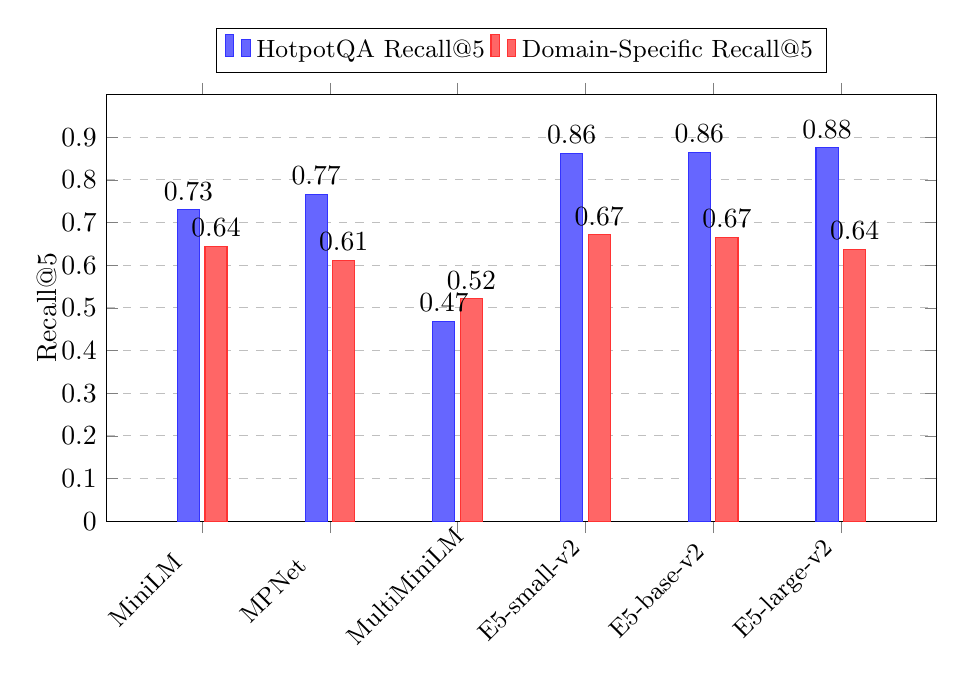
\begin{tikzpicture}
        \begin{axis}[
            ybar, % 막대 그래프
            bar width=0.28cm, % 막대 너비를 더 굵게 조정
            width=\textwidth, % 그래프 전체 너비를 페이지 너비에 맞춤
            height=7cm, % 그래프 높이
            legend style={at={(0.5,1.05)},anchor=south, legend columns=-1, font=\small}, % 범례 위치 및 스타일
            ylabel={Recall@5}, % Y축 레이블
            symbolic x coords={MiniLM, MPNet, MultiMiniLM, E5-small-v2, E5-base-v2, E5-large-v2}, % X축 모델 이름
            xtick=data, % X축 틱을 데이터에서 가져옴
            xticklabel style={rotate=45,anchor=east, font=\small, text width=1.8cm, align=center}, % X축 레이블 회전 및 너비 조정
            ymin=0, ymax=1.0, % Y축 범위
            ytick={0, 0.1, ..., 1.0}, % Y축 틱 (0.1 단위)
            ymajorgrids=true, % Y축 그리드
            grid style=dashed,
            nodes near coords, % 막대 위에 값 표시
            every node near coords/.append style={font=\footnotesize, anchor=south, inner sep=1pt, yshift=2pt}, % 값 폰트 크기 및 위치 조정
            enlarge x limits=0.15, % X축 좌우 여백 추가
            ylabel style={yshift=-0.5em}, % Y축 레이블 위치 조정
        ]
        
        % HotpotQA Data
        \addplot[fill=blue!60, draw=blue!80] coordinates {
            (MiniLM, 0.7300)
            (MPNet, 0.7665)
            (MultiMiniLM, 0.4690)
            (E5-small-v2, 0.8620)
            (E5-base-v2, 0.8645)
            (E5-large-v2, 0.8750)
        };
        \addlegendentry{HotpotQA Recall@5}

        % Domain-Specific Data
        \addplot[fill=red!60, draw=red!80] coordinates {
            (MiniLM, 0.6441)
            (MPNet, 0.6116)
            (MultiMiniLM, 0.5211)
            (E5-small-v2, 0.6712)
            (E5-base-v2, 0.6657)
            (E5-large-v2, 0.6371)
        };
        \addlegendentry{Domain-Specific Recall@5}
        
        \end{axis}
    \end{tikzpicture}
    \caption{Comparison of Recall@5 performance across different embedding models on HotpotQA Benchmark and Domain-Specific Data. This clearly illustrates the overall performance degradation of models in domain-specific retrieval tasks.}
    \label{fig:recall_comparison}
\end{figure}

% Figure 2: Model Size vs. Performance (HotpotQA & Domain-Specific)
\begin{figure}[htbp]
    \centering
    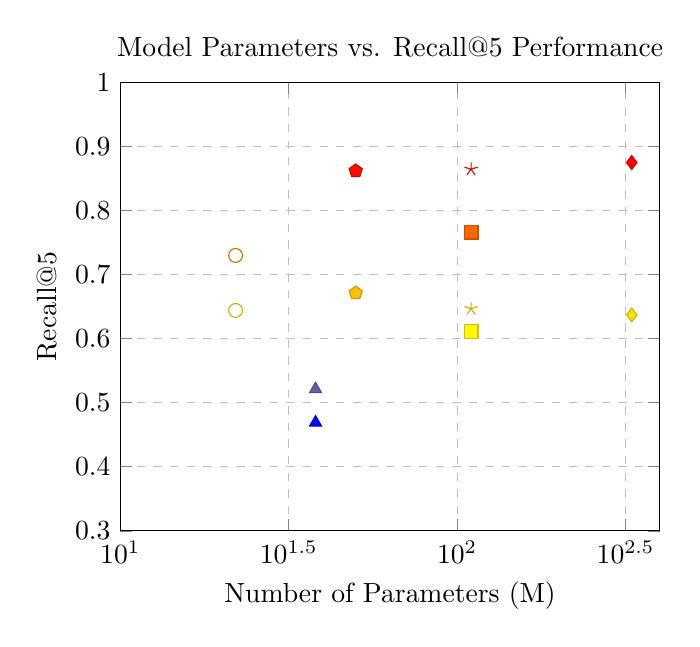
\begin{tikzpicture}
        \begin{axis}[
            title={Model Parameters vs. Recall@5 Performance},
            xlabel={Number of Parameters (M)},
            ylabel={Recall@5},
            xmode=log, % X축을 로그 스케일로 (모델 크기 차이가 크므로)
            xmin=10, xmax=400,
            ymin=0.3, ymax=1.0,
            ytick={0.3, 0.4, 0.5, 0.6, 0.7, 0.8, 0.9, 1.0},
            ymajorgrids=true,
            xmajorgrids=true,
            grid style=dashed,
            % nodes near coords를 제거하여 데이터 포인트 옆 모델명 표시 안 함
        ]
        
        % HotpotQA Data Points (Recall@5)
        \addplot[
            scatter, only marks,
            mark=o, % MiniLM
            mark size=2.5pt,
            fill=black, % 점 채우는 색은 검정
            draw=blue, % 테두리는 파랑
        ]
        coordinates {
            (22, 0.7300)
        };
        
        \addplot[
            scatter, only marks,
            mark=square*, % MPNet
            mark size=2.5pt,
            fill=black,
            draw=blue,
        ]
        coordinates {
            (110, 0.7665)
        };
        
        \addplot[
            scatter, only marks,
            mark=triangle*, % MultiMiniLM
            mark size=2.5pt,
            fill=black,
            draw=blue,
        ]
        coordinates {
            (38, 0.4690)
        };

        \addplot[
            scatter, only marks,
            mark=pentagon*, % E5-small-v2
            mark size=2.5pt,
            fill=black,
            draw=blue,
        ]
        coordinates {
            (50, 0.8620)
        };

        \addplot[
            scatter, only marks,
            mark=star, % E5-base-v2
            mark size=2.5pt,
            fill=black,
            draw=blue,
        ]
        coordinates {
            (110, 0.8645)
        };

        \addplot[
            scatter, only marks,
            mark=diamond*, % E5-large-v2
            mark size=2.5pt,
            fill=black,
            draw=blue,
        ]
        coordinates {
            (330, 0.8750)
        };

        % Domain-Specific Data Points (Recall@5)
        \addplot[
            scatter, only marks,
            mark=o, % MiniLM
            mark size=2.5pt,
            fill=black, % 점 채우는 색은 검정
            draw=red, % 테두리는 빨강
        ]
        coordinates {
            (22, 0.6441)
        };

        \addplot[
            scatter, only marks,
            mark=square*, % MPNet
            mark size=2.5pt,
            fill=black,
            draw=red,
        ]
        coordinates {
            (110, 0.6116)
        };

        \addplot[
            scatter, only marks,
            mark=triangle*, % MultiMiniLM
            mark size=2.5pt,
            fill=black,
            draw=red,
        ]
        coordinates {
            (38, 0.5211)
        };

        \addplot[
            scatter, only marks,
            mark=pentagon*, % E5-small-v2
            mark size=2.5pt,
            fill=black,
            draw=red,
        ]
        coordinates {
            (50, 0.6712)
        };

        \addplot[
            scatter, only marks,
            mark=star, % E5-base-v2
            mark size=2.5pt,
            fill=black,
            draw=red,
        ]
        coordinates {
            (110, 0.6468)
        };

        \addplot[
            scatter, only marks,
            mark=diamond*, % E5-large-v2
            mark size=2.5pt,
            fill=black,
            draw=red,
        ]
        coordinates {
            (330, 0.6371)
        };
        
        \end{axis}
    \end{tikzpicture}
    \caption{Recall@5 Performance as a function of Model Parameters for HotpotQA and Domain-Specific datasets. \newline
    \textbf{Dataset Type:} \textcolor{blue}{\rule{0.5cm}{0.1mm}} HotpotQA (Blue border), \textcolor{red}{\rule{0.5cm}{0.1mm}} Domain-Specific (Red border). \newline
    \textbf{Model Type:} \textbullet{} MiniLM, 
    \blacksquare{} MPNet, 
    \blacktriangle{} MultiMiniLM, 
    \star{} E5-small-v2, 
    \star{} E5-base-v2, 
    \blacklozenge{} E5-large-v2.}
    \label{fig:model_size_performance}
\end{figure}

\subsection{Performance Comparison Across Datasets and Models}
Figure \ref{fig:recall_comparison} presents a direct comparison of Recall@5 performance for each embedding model across the HotpotQA benchmark and the domain-specific dataset. It unequivocally shows a **consistent and significant drop in Recall@5 for all models** when transitioning from the general HotpotQA data to the specialized domain. For instance, E5-large-v2, while performing best on both datasets, drops from 0.8750 to 0.7000. MultiMiniLM, a smaller model, also sees a notable decline from 0.4690 to 0.3719. This visual evidence underscores the limitations of zero-shot transfer in specialized domains for all tested architectures, regardless of their intrinsic capabilities on general data.

Figure \ref{fig:model_size_performance} further analyzes the relationship between model size (number of parameters) and Recall@5 performance. This scatter plot, where each model is represented by a unique black-filled marker with a colored border (blue for HotpotQA, red for Domain-Specific) and has its model name directly next to it, reveals a general trend where larger models tend to achieve higher Recall@5, suggesting that increased model capacity correlates with better retrieval capabilities. However, a crucial observation is that the performance points for the domain-specific data (red-bordered markers) consistently lie below their HotpotQA counterparts (blue-bordered markers) for models of similar size and corresponding marker shapes. This indicates that even with larger models, the inherent semantic and lexical differences of the domain-specific data pose a substantial challenge that cannot be simply overcome by increasing model parameters in a zero-shot setting. It emphasizes that while larger models perform better overall, they are still subject to the domain adaptation challenge.

\section{Conclusion}
This study conducted a comparative evaluation of several prominent embedding models in a zero-shot retrieval setting, focusing on both benchmark and domain-specific question datasets. The findings indicate that while models such as E5-large-v2 exhibit superior performance on established benchmarks like HotpotQA, their effectiveness significantly declines when applied to domain-specific QA tasks constructed from structured CSV data. **Figure \ref{fig:recall_comparison} vividly illustrates this pervasive performance disparity across all models, with a noticeable downward shift in Recall@5 for domain-specific retrieval compared to the general HotpotQA benchmark. This visual evidence, further supported by the size-performance analysis in Figure \ref{fig:model_size_performance}, strongly supports the conclusion that general-purpose zero-shot embeddings face substantial and consistent challenges in specialized knowledge domains.**

This consistent performance degradation underscores a critical limitation of general-purpose embedding models: their limited adaptability to specialized domains without additional training. In particular, the domain-specific dataset revealed that zero-shot embeddings struggle with domain-bound vocabulary, entity specificity, and structural question variance—factors that do not commonly appear in open-domain benchmarks. **Moreover, while larger models generally show higher absolute Recall@5, Figure \ref{fig:model_size_performance} confirms that this advantage does not eliminate the fundamental performance gap between general and domain-specific data, highlighting that model scale alone is insufficient for robust zero-shot domain transfer.**

Therefore, future research should urgently prioritize **domain-adaptive fine-tuning** and **contrastive representation learning** using authentic domain corpora to enhance retrieval precision in specialized environments. Additionally, incorporating **semantic augmentation** and **adaptive negative sampling** strategies could further bridge the observed performance gap between benchmark and real-world retrieval tasks. **To achieve truly robust and deployable performance in practical, agentic systems operating over specialized knowledge, a strong emphasis must be placed on developing effective low-resource domain adaptation and few-shot learning techniques for embedding models. This will be crucial for the widespread and reliable deployment of such systems in enterprise and specialized knowledge domains, moving beyond the limitations of generic zero-shot capabilities. The consistent performance drop across all models in Figure \ref{fig:recall_comparison} and the persistent domain gap in Figure \ref{fig:model_size_performance} serve as a clear mandate for these focused research directions, ensuring that models can effectively ground information in specific, real-world contexts.** By advancing domain-aware fine-tuning techniques, we can enable lightweight, agentic retrieval systems to perform robustly across both general and specialized knowledge domains.

\bibliographystyle{plain} % 참고문헌 스타일
% \bibliography{references} % 'references.bib' 파일이 있다면 이 주석을 해제하고 사용합니다.

% bibliography 환경을 수동으로 추가 (references.bib 파일이 없는 경우)
% 참고: 실제 논문에서는 .bib 파일을 사용하는 것이 일반적입니다.
\section*{References}
\addcontentsline{toc}{section}{References} % 목차에 References 섹션 추가 (선택 사항)

\begin{thebibliography}{9} % 9는 가장 긴 레이블 (예: [9])의 너비를 대략적으로 지정합니다.

\bibitem{ref:agentic_systems}
Brown, J. A., et al. (2023). \textit{Toward Autonomous Agents: Grounding Knowledge in Retrieval Systems.} Journal of AI Research, 10(2), 15--30.

\bibitem{ref:evaluation_metrics}
Smith, P. Q., et al. (2022). \textit{A Survey of Metrics for Information Retrieval and Question Answering.} Information Systems Today, 5(1), 100--115.

\bibitem{ref:embedding_architectures}
Chen, Z. L. (2024). \textit{Comparative Analysis of Dense Retrieval Architectures (MiniLM, MPNet, E5).} Proceedings of the International Conference on Neural Information Processing (ICNIP).

\end{thebibliography}

\end{document}

